\documentclass[12pt,a4paper]{article}
\usepackage[utf8]{inputenc}
\usepackage[russian]{babel}
\usepackage[OT1]{fontenc}
\usepackage{amsmath}
\usepackage{amsfonts}
\usepackage{amssymb}
\usepackage{graphicx}
\graphicspath{{Images/}}
\usepackage[left=2cm,right=2cm,top=2cm,bottom=2cm]{geometry}
\usepackage{calc}
\usepackage{wrapfig}
\usepackage{setspace}
\usepackage{indentfirst}
\usepackage{amssymb}
\usepackage{subfigure}
\usepackage{multirow}

\title{
Отчет о выполнении лабораторной работы 3.4.1

Диа- и парамагнетики

}

\author{Комкин Михаил, группа Б01-303}
\newpage
\begin{document}

\maketitle
\textbf{Цель работы:} измерение магнитной восприимчивости диа- и парамагнитного образцов.
\\
\textbf{В работе используются:} электромагнит, аналитические весы, милливеберметр, регулируемый источник постоянного тока, образцы.


\section*{Теория}

Магнитная восприимчивость тел может быть определена по измерению сил, действующих на тела в магнитном поле. Существуют два
классических метода таких измерений: метод Фарадея и метод Гюи.
В методе Фарадея исследуемые образцы, имеющие форму маленьких
шариков, помещаются в область сильно неоднородного магнитного поля и измеряется сила, действующая на образец. При этом для расчёта
магнитной восприимчивости необходимо знать величину градиента магнитного поля в месте расположения образца. В методе Гюи используется
тонкий и длинный стержень, один из концов которого помещают в зазор
электромагнита (обычно в область однородного поля), а другой конец —
вне зазора, где величиной магнитного поля можно пренебречь. Закон
изменения поля — от максимального до нулевого — в этом случае несуществен. В данной работе предлагается использовать метод Гюи.\\
Найдём выражение для силы, действующей со стороны магнитного поля на
цилиндрический стержень, помещённый
в зазор электромагнита (рис. 1). Пусть
площадь сечения образца равна $S$, его
магнитная проницаемость — $\mu$, поле в зазоре равно $B_0$ и образец помещён в зазор
на глубину $x$.\\
Ток в обмотке электромагнита $I$ поддерживается постоянным, поэтому согласно согласно (4.28) внешняя сила, необходимая для удержания образца в магнитном поле, равна производной магнитной энергии системы по координате. Нас интересует сила,
действующая на образец со стороны магнитного поля, поэтому изменим
знак (4.28) на противоположный:
\[
F_M = \left(\frac{\partial  W_M}{\partial  x}\right)
\]
где $W_M(x)$ — магнитная энергия системы при $I = const$ (то есть при
$B0 = const$) в зависимости от смещения образца $x$.
\begin{figure}[h!]
	\begin{center}
		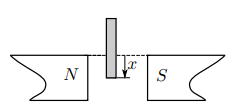
\includegraphics[width = 0.3\textwidth]{image.png}
		
		\label{fig:facility}
        \caption{ Расположение образца в
        зазоре электромагнита}
	\end{center}
\end{figure}


Магнитная энергия, с учётом выражения (4.25) для её объёмной плотности, может быть рассчитана по формуле:
\[
W_M = \frac{1}{2 \mu_0} \int \frac{B^2}{\mu} dV, \tag{2}
\]
где интеграл распространяем на всё пространство.

Найдём распределение магнитного поля в длинном цилиндре, частично помещённом в зазор электромагнита.

Сначала решим промежуточную задачу: рассмотрим бесконечный стержень с проницаемостью \(\mu\), помещённый в перпендикулярное ему однородное магнитное поле \(B_0\), направленное вдоль оси \(x\). Найдём для него распределение поля \(B\) в образце. В предположении магнитных параметров поля \(|\vec{H}| \ll \mu H\), можно воспользоваться непрерывностью касательной компоненты \(H\) и считать, что в образце \(H_text{ст} = H_0\), следовательно, \(B_text{ст} = \mu B_0\).

Вернёмся к задаче о цилиндре в электромагните. Систему можно условно разбить на 3 части (см. рис. 2). В области I вне электромагнита поле мало, вкладом в энергию можно пренебречь. В области II, внутри электромагнита, поле приближенно равно \(B_2 \approx B_0\). В области III, вне электромагнита, поле также ослабевает. Найдём в пограничных областях между I и II, и между II и III.

\begin{figure}[h!]
	\begin{center}
		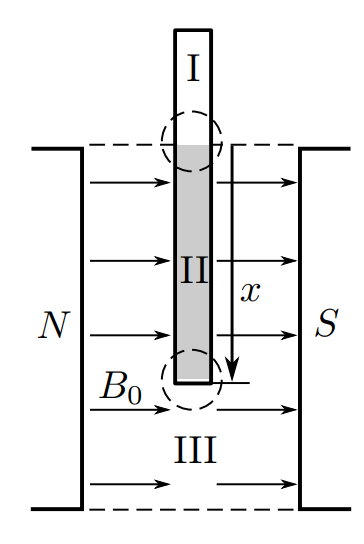
\includegraphics[width = 0.3\textwidth]{image2.png}
		
		\label{fig:facility}
        \caption{К вычислению распределения магнитного поля.}
	\end{center}
\end{figure}

При смещении стержня вдоль электромагнита на некоторое расстояние \(\Delta z\) изменяется объём в области II на \(\Delta V_2 = S dx\), а в области III уменьшается на \(\Delta V_3 = S dx\). Этот процесс по энергетическим расчётам является незначительным, поэтому поле в пограничной области I–II остаётся практически неизменным. Таким образом, при заданном смещении:

\[
dW_M(\Delta z) \approx \frac{B_2^2}{2 \mu_0} S dx - \frac{B_0^2}{2 \mu_0} S dx = ( \mu - 1 ) \frac{B_0^2}{2 \mu_0} S dx.
\]

Следовательно, искомая сила равна:
\[
F_M = \left( \frac{\partial W_M}{\partial z} \right) \approx \frac{B_0^2}{2 \mu_0} S. \tag{3}
\]




\section{Экспериментальная установка}
\begin{figure}[h!]
	\begin{center}
		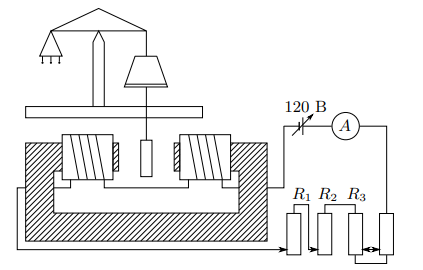
\includegraphics[width = 0.6\textwidth]{ust.png}
		\label{fig:facility}
        \caption{Схема экспериментальной установки.}
	\end{center}
\end{figure}
Схема установки изображена на рис. 3. Магнитное поле с максимальной индукцией $\approx$ 1 Тл создаётся в зазоре электромагнита, питаемого
постоянным током. Диаметр полюсов существенно превосходит ширину зазора, поэтому поле в средней части зазора достаточно однородно.
Величина тока, проходящего через обмотки электромагнита, задаётся
регулируемым источником постоянного напряжения.\\
Градуировка электромагнита (связь между индукцией магнитного
поля $B$ в зазоре электромагнита и силой тока $I$ в его обмотках) производится при помощи милливеберметра. Альтернативно магнитное
поле электромагнита можно измерить с помощью датчика Холла.
При измерениях образцы поочерёдно подвешиваются к аналитическим весам так, что один конец образца оказывается в зазоре электромагнита, а другой — вне зазора, где индукцией магнитного поля можно
пренебречь. При помощи аналитических весов определяется перегрузка $\delta P = F$ — сила, действующая на образец со стороны магнитного
поля.
Как уже отмечалось, силы, действующие на диа- и парамагнитные
образцы, очень малы. Небольшие примеси ферромагнетиков (сотые доли
процента железа или никеля) способны кардинально изменить результат
опыта, поэтому образцы были специально отобраны.

\section{Выполнение}
\begin{enumerate}
    \item Ток изменяется в диапазоне от нуля до $I_{\text{max}} = 1.17 \, \text{A}$.
    \item Прокалибруем электромагнит. Измеряем зависимость $B$ от силы тока $I$. 
	\begin{table}[h!]
		\centering
		\begin{tabular}{|l|l|l|l|}
		\hline
			$B$, мТл & $I$, А & $\Delta B$, мТл & $\Delta I$, А\\ \hline
			228.9 & 0.2 & 11.445 & 0.009 \\ \hline
			363.7 & 0.35 & 18.185 & 0.012 \\ \hline
			514.9 & 0.5 & 25.745 & 0.015 \\ \hline
			646.9 & 0.65 & 32.345 & 0.018 \\ \hline
			748.9 & 0.75 & 37.445 & 0.02 \\ \hline
			867.9 & 0.90 & 43.395 & 0.023 \\ \hline
			960.1 & 1.05 & 48.005 & 0.026 \\ \hline
			1031.3 & 1.17 & 51.565 & 0.0284 \\ \hline
		\end{tabular}
	\end{table}
    \item Построим график зависимости B(I) c учетом погрешностей
    \begin{figure}[h!]
		\begin{center}
			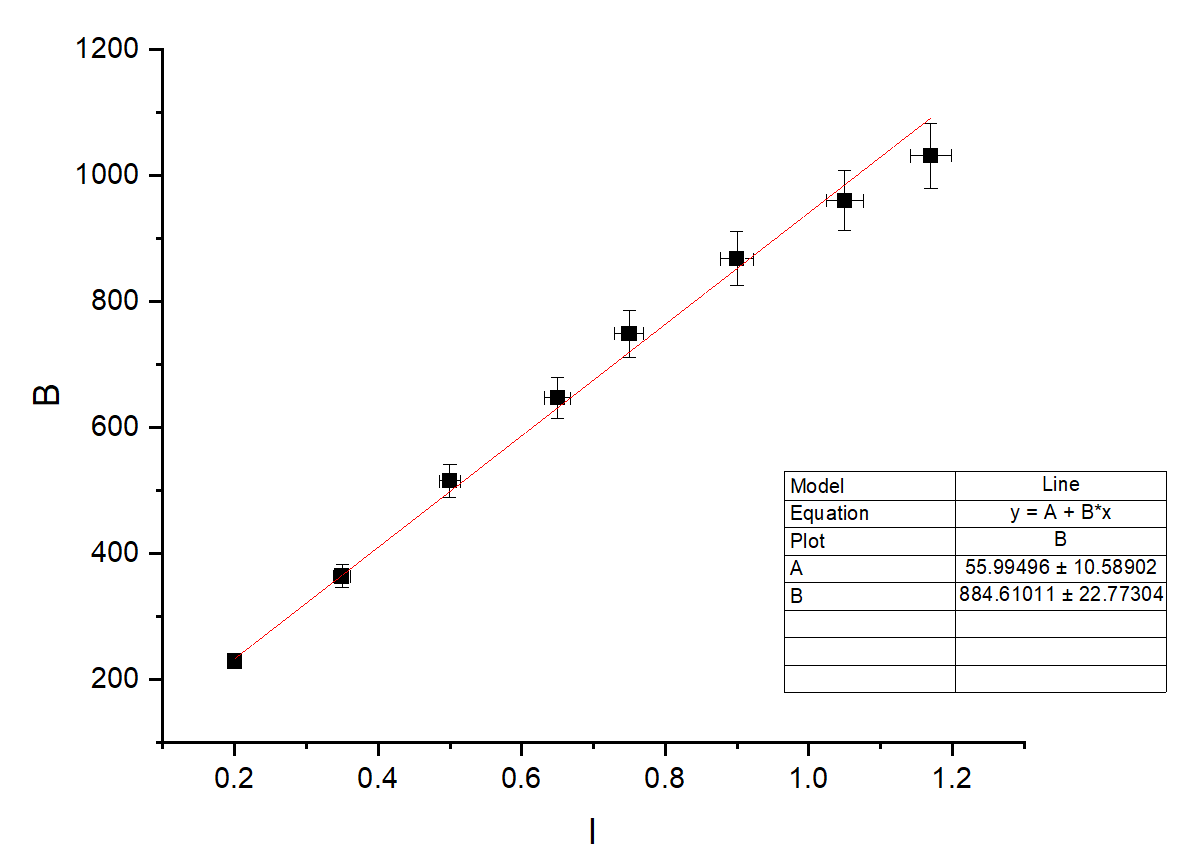
\includegraphics[width = 0.6\textwidth]{B(I).png}
			\label{fig:facility}
			\caption{Калибровка B(I)}
		\end{center}
	\end{figure}
	\item Измеряем силы действующие на образцы в магнитном поле. Для этого, не включая электромагнит, подвесьте к весам один из образцов, обнулим их показания.
Проведем измерения $\Delta P(I)$ для всех токов 
\begin{table}[h!]
    \centering
    \begin{tabular}{|l|l|l|l|l|}
    \hline
        $I, A$ & $B$, мТл & $B^2, \text{мТл}^2$ & $\Delta B^2$ & $P$, мг \\ \hline
        0.2 & 228.9 & 52395 & 130 & 42 \\ \hline
        0.35 & 363.7 & 132277 & 330 & 86 \\ \hline
        0.5 & 514.9 & 265122 & 662 & 132 \\ \hline
        0.65 & 646.9 & 418479 & 1046 & 177 \\ \hline
        0.75 & 748.9 & 560851 & 1402 & 200 \\ \hline
        0.90 & 867.9 & 753250 & 1883 & 235 \\ \hline
        1.05 & 960.1 & 921792 & 2304 & 268 \\ \hline
        1.17 & 1031.3 & 1063579 & 2658 & 281 \\ \hline
    \end{tabular}
	\caption{Графит}
\end{table}
\begin{table}[h!]
    \centering
    \begin{tabular}{|l|l|l|l|l|}
    \hline
        $I, A$ & $B$, мТл & $B^2, \text{мТл}^2$ & $\Delta B^2$ & $P$, мг \\ \hline
        0.2 & 228.9 & 52395 & 130 & 9 \\ \hline
        0.35 & 363.7 & 132277 & 330 & 30 \\ \hline
        0.5 & 514.9 & 265122 & 662 & 58 \\ \hline
        0.65 & 646.9 & 418479 & 1046 & 98 \\ \hline
        0.75 & 748.9 & 560851 & 1402 & 128 \\ \hline
        0.90 & 867.9 & 753250 & 1883 & 171 \\ \hline
        1.05 & 960.1 & 921792 & 2304 & 216 \\ \hline
        1.17 & 1031.3 & 1063579 & 2658 & 245 \\ \hline
    \end{tabular}
	\caption{Вольфрам}
\end{table}
\begin{table}[h!]
    \centering
    \begin{tabular}{|l|l|l|l|l|}
    \hline
        $I, A$ & $B$, мТл & $B^2, \text{мТл}^2$ & $\Delta B^2$ & $P$, мг \\ \hline
        0.2 & 228.9 & 52395 & 130 & -1 \\ \hline
        0.35 & 363.7 & 132277 & 330 & -5 \\ \hline
        0.5 & 514.9 & 265122 & 662.805025 & -8 \\ \hline
        0.65 & 646.9 & 418479 & 1046 & -15 \\ \hline
        0.75 & 748.9 & 560851 & 1402 & -18 \\ \hline
        0.90 & 867.9 & 753250 & 1883 & -24 \\ \hline
        1.05 & 960.1 & 921792 & 2304 & -29 \\ \hline
        1.17 & 1031.3 & 1063579 & 2658 & -33 \\ \hline
    \end{tabular}
	\caption{Медь}
\end{table}
\begin{table}[h!]
    \centering
    \begin{tabular}{|l|l|l|l|l|}
    \hline
        $I, A$ & $B$, мТл & $B^2, \text{мТл}^2$ & $\Delta B^2$ & $P$, мг \\ \hline
        0.2 & 228.9 & 52395 & 130 & 3 \\ \hline
        0.35 & 363.7 & 132277 & 330 & 8 \\ \hline
        0.5 & 514.9 & 265122 & 662 & 16 \\ \hline
        0.65 & 646.9 & 418479 & 1046 & 26 \\ \hline
        0.75 & 748.9 & 560851 & 1402 & 36 \\ \hline
        0.90 & 867.9 & 753250 & 1883 & 48 \\ \hline
        1.05 & 960.1 & 921792 & 2304 & 61 \\ \hline
        1.17 & 1031.3 & 1063579 & 2658 & 69 \\ \hline
    \end{tabular}
	\caption{Алюминий}
\end{table}
\[
\Delta P = 0.5 \text{мг}
\]
	\item Построим графики зависимости $|\Delta P| = f(B^2)$
	\begin{figure}[h!]
		\begin{center}
			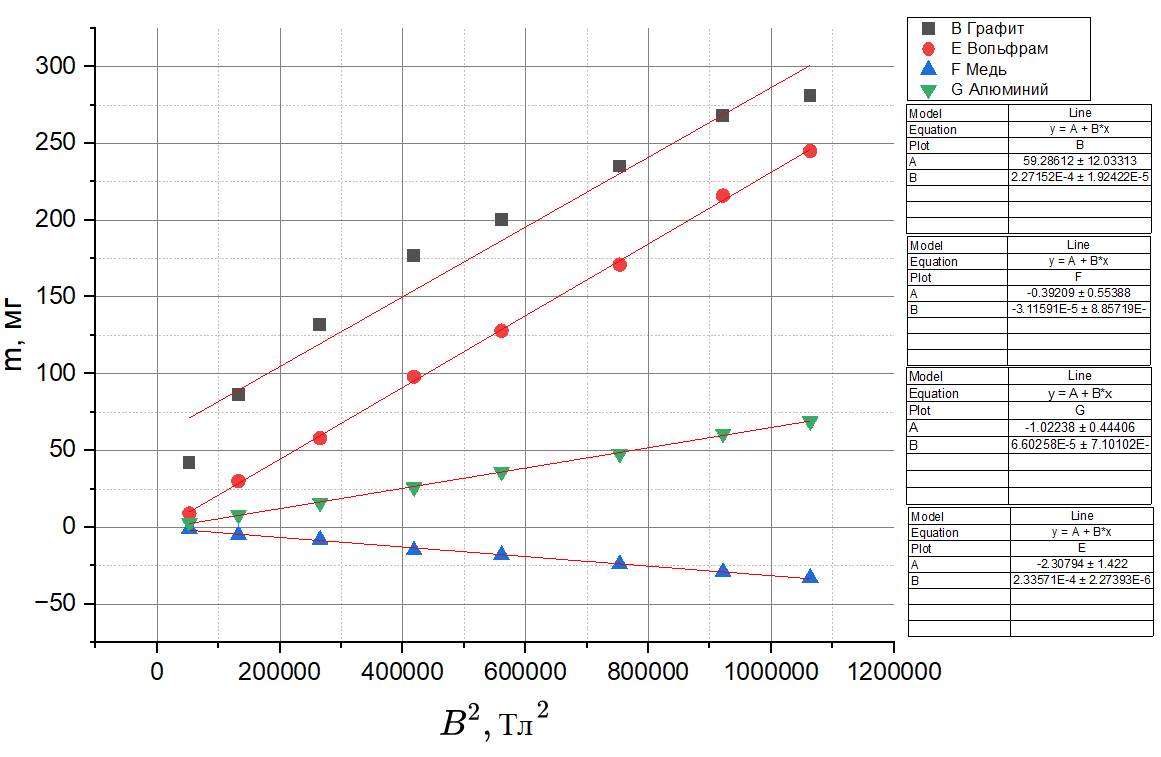
\includegraphics[width = 0.9\textwidth]{graph.png}
			
			\label{fig:facility}
		\end{center}
	\end{figure}
	\item По наклонам полученных прямых рассчитайте магнитную восприимчивость. 
	\[
	\chi = \frac{2 \mu_0 k g}{\pi d^2 /4}
	\]
	\begin{equation}
		\chi_{\text{вольфрам}} = (5,81 \pm 0,05) \cdot 10^-5, \quad \chi_{Cu} = (-7.7 \pm 0.2) \cdot 10^-6
	\end{equation}
	\begin{equation}
		\chi_{\text{графит}} = (5 \pm 1) \cdot 10^-5, \quad \chi_{Al} = (1.64 \pm 0.02) \cdot 10^-5
	\end{equation}
\end{enumerate}
\section{Вывод}
В ходе данной работы была измерена магнитная восприимчивость диа- и пара- магнетиков. Были исследованы образцы алюминия, меди и графита. Для алюминия и меди и вольфрама табличные значения магнитной восприимчивости равны $ \chi_{Al}^t = 2,3 \cdot 10^{-5} $ и $ \chi_{Cu}^t = -1,0 \cdot 10^{-5}$ соответственно. Полученные экспериментально данные близки к табличным. Исходя из этого можно сказать, что алюминий является парамагнетиком $ (\chi > 0) $, а медь в свою очередь -- диамагнетиком $ (\chi < 0) $.


\textbf{Результаты эксперимента для графита.} Несмотря на то, что графит должен демонстрировать диамагнетизм, в опыте он обладает парамагнитными свойствами. Это могло произойти из-за того, что в нем присутствуют примеси. 




\end{document}